%% uctest.tex 11/3/94
%% Copyright (C) 1988-2004 Daniel Gildea, BBF, Ethan Munson.
%
% This work may be distributed and/or modified under the
% conditions of the LaTeX Project Public License, either version 1.3
% of this license or (at your option) any later version.
% The latest version of this license is in
%   http://www.latex-project.org/lppl.txt
% and version 1.3 or later is part of all distributions of LaTeX
% version 2003/12/01 or later.
%
% This work has the LPPL maintenance status "maintained".
% 
% The Current Maintainer of this work is Daniel Gildea.
%
% 2007/08/01
% LaTeX Package "ucr" is modified from LaTeX package "ucthesis."
% This modification is therefore under to the conditions of 
% the LaTeX Project Public License.
% Its formality is suitable for the dissertation of Universty of
% California, Riverside.
% This test document is for the convenience of all students of
% Universty of California, Riverside.
% Contact Charles Yang at chcyang@yahoo.com if you like.
% Charles Yang has nothing to do with the original author's sarcasm.
%
% \documentclass[11pt]{ucthesis}
% \documentclass[11pt]{ucr}
\documentclass[oneside,final, letterpaper]{ucr}
\begin{document}

% Declarations for Front Matter

\title{MEASUREMENT OF THE LONGTIDUDIANL SINGLE SPIN ASYMMETRY, $A_L$, FOR POLARIZED PROTON-PROTON COLLISIONS IN THE $W\rightarrow\mu$ DECAY CHANNEL}
\author{Michael J. Beaumier}
\degreemonth{August}
\degreeyear{2016}
\degree{Doctor of Philosophy}
\chair{Professor Kenneth Barish }
\othermembers{Professor Rich Seto\\
Professor John Ellison}
\numberofmembers{3}
\field{Physics}
\campus{Riverside}

\maketitle
\copyrightpage{}
\approvalpage{}

\degreesemester{Summer}

\begin{frontmatter}

\begin{acknowledgements}
	Advisors and Mentors are some of the most important people any scientist will
encounter in their professional career. Time and again, I have heard colleagues
speak of "that one inspirational" person that drove them to be their best, and
knew how to "grow" a researcher. 

I am very greatful to my advisor, Ken Barish, whose calm, stoic and unabated
support helped guide me through my research. Ken involved me in many aspects of
the research group at UCR, beyond the scientific work. He insured that I was
exposed to all aspects of research in particle physics, including writing
grants, reviewing literature, mentoring younger students, building detectors,
running a particle accelelrator detector, and of course, data analysis.  Ken has
always had the uncanny ability to know "who to talk to" for nearly any problem I
might have. Ken connected me with other excellent physicists, who helped me grow
as a researcher, and he gave me the freedom I needed to pursue my interests, and
move in the scientific directions I felt most fruitful, while helping to provide
an overall direction for my academic career and research. 

Beyond all this, the single most important thing Ken has done for me, is to give
me a second chance in graduate school. When he accepted me into his group, I was
an undoubtedly risky choice. I struggled mightily my first year in grad school.
I earned poor grades, and even had to re-take a class. In fact, my performance
was so poor, that my teaching responsibilities were reduced, and eventually, I
lost my graduate division fellowship, which ultimately meant that I had no
income, or means of supporting myself; I was effectively dismissed from graduate
school. However, I was interested in the research carried out by Ken and Rich
Seto's heavy ion group, so I talked to Ken, who graciously accepted me into the
group, provided me with academic and financial support, and even flew me out to
Brookhaven National Lab my first summer of graduate school. I finally got to
dive into 'real' physics research. I think it was this vote of confidence from
Ken, as well as the awesome physics happening at the PHENIX experiment which
gave me the confidence to wholeheartedly devote myself to my studies and
research. Without Ken's vote of confidence, I fear that my graduate career would
have been over in short order.

While at Brookhaven National Lab, I encountered graduate students, post docs,
research staff, and other amazing physicists who taught me an incredible
amount, and showed both patience, kindess, friendship and mentorship to me.
Richard Hollis was one of the first people I encoutered in my research group at
UCR - I have never met a more patient person. Richard helped me get my
bearings, and set me straight, during my early (and later) years of graduate
school. Oleg Eyser was with our group at that time as well - although I recall
that he was less than thrilled to have yet another green graduate student
constantly asking questions, taking time away from his work. He still made time
to teach me, and introduced me to the very complicated PHENIX software system.
Oleg challenged me, and expected me to find answers for myself, and was
unrelenting in that regard, which I am certain made me a better researcher.

Josh Perry gave me a crash course on the PHENIX data acquisition system,
boiling down this incredibly complicated system into understandable pieces, and
helped me learn that ultimately, persistance pays off when tackling difficult
problems. Martin Leitgab took me under his wing while I worked days and nights
to learn PHENIX's fast data production systems. Martin's systematic, calm, and
patient approach to problem solving has been something I have tried to emulate
since my work with him - I could not have asked for a better mentor for that
project. On that same project was my first introduction to Chris Pinkenburg and
Martin Purschke - somewhat of the yin and yang of the PHENIX online data
aquisition. I benefited enormously from conversations with both about PHENIX
software, and online systems. Martin Purschke's kindness and sense of humor
always spurred me on, while Chis' dogged dedication to doing things 'the right
way' kept me honest. I have returned to Martin with various questions many
times over the years, and he has always been cheerful, supportive and wise with
his answers. Probably nobody other than Ed Desmond has been woken up so many
times with emergencies at the PHENIX counting house in the middle of the night,
yet even when I woke him at 3 am on many occasions, would simply state, in an
execptionally dry, well practiced line: 'Martin Speaking, please state the
nature of your emergency'. I don't know of many who can manage to be coy and
good natured under such circumstances.

I have to acknoledge Joe Seele as well, in this regard, as he probably more
than anyone else, set me on the path to learning to program well, and using a
computer effectively - these skills, so often neglected in Particle Physics,
have paid off for me, many, many times over.

W Analysis Crew \\
  Ralf Seidl, 
  Francesca Giordano, 
  Sangwha Park, 
  Daniel Jumper, 
  Abraham Meles,
  Chong Kim, 

Friends and Family \\
  Bob Beaumier, 
  Marian Beaumier, 
  Joe Beaumier, 
  David Beaumier, 
  Emily Vance, 
  Jackie Hubbard, 
  Alexander Anderson-Natalie, 
  Corey Kownacki, 
  Chris Heidt, 
  Pat Odenthal, 
  Behnam Darvish Sarvestani, 
  Oleg Martynov, 

\end{acknowledgements}

\begin{dedication}
\null\vfil
{\large
\begin{center}
	Some say that it takes a village to raise a child. The same can be said of
	raising a graduate student up to earning a PhD. This thesis is dedicated to
	the multitude who have helped me become the man I am today, and to students
	who struggle, and their mentors who do not give up on them. \\
\end{center}}
\vfil\null
\end{dedication}

\begin{abstract}
	This thesis discusses the process of extracting information about the spin
	structure of protons, specifically, spin contributions from the sea of quarks
	and antiquarks, which are kinematically distinct from the 'valence quarks'. We
	have known since the 'proton-spin crisis' ~\cite{1988PhLB..206..364A} of the 1990s that proton
	spin does not entirely reside in the valence quarks, so the thurst of
	experimental efforts since then have been designed to determine both how to
	probe the proton spin structure, and how to validate models for proton spin
	structure. Here, I discuss one particular approach to understanding the
	sea-quark spin contribution, which utilizes the production of real $W$-bosons,
	and the $W$ coupling with polarized spin structure in the proton sea, as
	produced from polarized protons collisions.  Only one of the colliding protons
	is longitudinally spin polarized, in this analysis, and they are collided at
	an energy of $500 GeV$. The expermental observable used is referred to as
	"$A_L$" which is expressed mathematically as a ratio of sums and differences
	of various helicity combinations of singly polarized interactions between two
	protons, i.e.  $p+p^{\Rightarrow}: \rightarrow W \rightarrow \mu + \nu$. Once
	$A_L$ has been experimentally measured, it can then be used to determine
	appropriate polarizations of proton sea-quarks, within a given uncertainty, if
	we write the cross-sections used in the calculation of $A_L$ in terms of
	polarized parton distribution functions. Finally, this thesis will also
	include a discussion of my work experimentally determining the absolute
	luminosity of collisions at RHIC, which is needed as a normalization on any
	cross section used in the analysis. In particular, studying the cross section
	of the $W$ interaction can help to validate our models for assigning a
	signal-to-background ratio to the $W\rightarrow\mu$ events.  
\end{abstract}


\tableofcontents
\listoffigures
\listoftables
\end{frontmatter}

% \part{First Part}


\chapter{Introduction}

\section{A Brief History of the Proton}
The angular momentum of the proton has been a subject of study for the last 20
years\needcite{}. One of the challenges of particle physics is to create a
framework which can accurately describe matter, as well as predict the behavior
of matter at all energy scales. The proton is a baryon which makes up the
majority of the mass in the visible universe, yet fully understanding the
origins of its properties - such as its mass and spin, still eludes us. However,
through the applicaiton of the scientific method over many generations of
physicists, we have magnificently described this important particle, and
understood much of its properties. However, one property which still defies our
descriptions is its fundamental angular momentum, spin. \\
	
Our understanding of the proton has evolved and sharpened since the first
experiments in deep inelastic scattering showed that the proton is not a
fundamental particle~\cite{Breidenbach1969}. Gell-Mann later planted the
seeds of a theoretical framework which could in part describe some of the
structure of baryons, a class of hadrons which we may naively describe as
composed of three 'valence quarks'\needcite{}. We can apply well known spin-sum
rules to the indivdual spins of the valence quarks which compose the proton in
our naive valence-model to produce a correct prediction for the protons' spin
${1}\over{2}$. When experimenters set out to measure the contribution of these
valence quarks in 1988 at the EMC experiment~\cite{Ashman1988}, they
were flabbergasted to find that the valence quarks carry only a small fraction
of the proton's spin. Although recent papers~\cite{Povh2016} suggest that this 'spin
crisis' is simple due to misattribution of spin, most literature to date has
focused on understanding how to model the proton with parton distribution
functions. These parton distribution functions come in many varieties, and probe
different degrees of freedom within the proton, in both the case of unpolarized
partion distribution funcitons, and polarized parton distribution functions. \\
 
\section{Scope and Objectives of This Work}
This thesis will describe the research I carried out between May of 2010 through
August of 2016. I will often quote work that was carried out in active
collaboration with Ralf Seidel, Francesca Giordano, Daniel Jumper, Sanghwa Park,
Abraham Meles and Chong Kim. Daniel, Abraham, Ralf, Francesca, and myself all
worked on the 2013 polarized proton data set taken at RHIC with PHENIX. This
analysis comprises the body of work devoted to calculating $A_L$ for the
$W\rightarrow\mu$ decay. Since 2013, the five of us collaborated closely on all
aspects of the work, which provided invaluable cross-checks at nearly every
stage. Many of the figures in this document were produced by our collective
efforts, and I will do my best to cite when possible, if one analyzer played a
particularly large role in generating the data or visualization, however after
several years of working together, I will certainly fail to attribute, or
misattribute at times.

The other portion of this thesis will discuss the Vernier Analysis, which is
instrumental for every single-cross-section calculation taken with RHIC data.
The thrust of the Vernier Analysis is to determine the beam luminosity at
PHENIX's interaction point, so as to normalize these cross-section calculations.
This is done with a series of specialized Vernier-Scans, where beams are scanned
across one-another in order to measure beam geometry. The luminosity can then be
calcualted from first principals, and compared to the advertised machine
luminosity published by RHIC's collider-accelerator department. I began working
with the Vernier Analysis under the tutelage of K. Oleg Eyser, but eventually
moved to work independantly on the analysis, producing an entire software
framework for handling data cleaning, analysis, visualization and simulation.
 %usually intro
\chapter{Physics Background}
\section{The Phenomena of Spin}

Spin is a fundamental quantity possessed by all elementary particles. We use
the word 'spin' to describe the property, because partices which possess spin,
behave as though they have some kind of intrinsic, hidden rotation, as if they
were 'spinning'. The dimension of spin, therefore is angular momentum. What is
somewhat bizarre about spin, is that we do not observe anything physically
spinning - although there are some phenomena (such as oribtal angular momenta)
which can be naively thought of as a 'spinning system' (but this description
escapes classical analogy, due to its quantum, probibalistic nature). The role
of Spin in Physics is of foundational importance, and yet, we have not
succesfully produced a model which can accurately predict the spin of hadrons.

The presence of spin in relativistic particles creates the phenomona of
chriality, which has huge implications for how elementary particles can generate
structure in matter itself ~\needcite{}. In the case of the weak interaction,
the presence of spin, which creates Chiral spinors breaks the left-right
symmetry of weak coupling in matter (a fact which will be exploited in this
thesis to probe the spin of the proton sea).

The phenomena of spin also changes the rules for how ensembles of particles may
exist in a potential. Particles with spin are fermions, and because these
paritcles must obey fermi statistics, we can observe structure in matter in the
universe ~\needcite{}. Without spin, the world as we know would collapse on
itself, making any kind of extended non-exotic structures which currenlty exist
by virtue of the Pauli exclusion principal, impossible.

\section{A Brief History of Proton Spin}

The study of Spin is really just an outgrowth of the general study of matter.
Our models for matter, and the underlying structure of matter (in the modern
sense), represents over a hundred years of experimental and theoretical efforts,
and thousands of years of contemplating what makes up the universe.

Although indulgent on my part, I find it interesting, and humbling, to try and
map out the path that humanity and science has trodden on its way to
understanding the building blocks of the universe. To find the first time that
humanity had murmurings that suggested our visible world is built from
invisible, fundamental building blocks, we must travel back, nearly 2,500 years
into the past.

\subsection{Ancient Foundations}
Sometime around 490 - 370 BCE lived two philosophers, empedocles
(Fig~\ref{fig:empedocles}), and Democrtius (Fig~\ref{fig:democritus}). Both men
lived approximately at the same time, and made huge philosophical leaps in
attempting to understand the nature of the visible world.

\begin{figure}[h]
	\centering
	\begin{subfigure}{.5\textwidth}
		\centering
		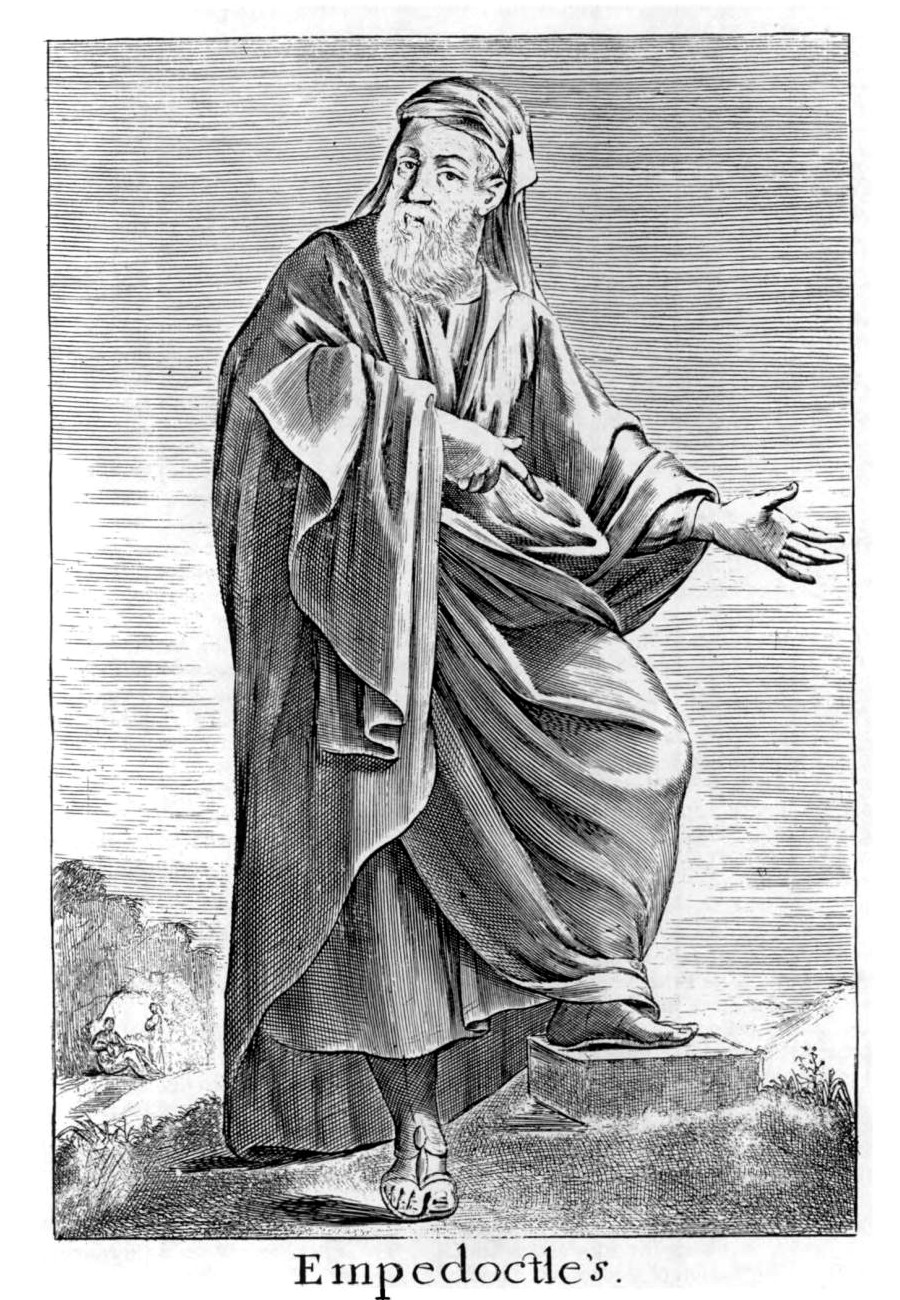
\includegraphics[width=0.4\linewidth]{../Chapter2/fig/empedocles.jpg}
		\caption{Empedocles}
		\label{fig:empedocles}
	\end{subfigure}%
	\begin{subfigure}{0.5\textwidth}
		\centering
		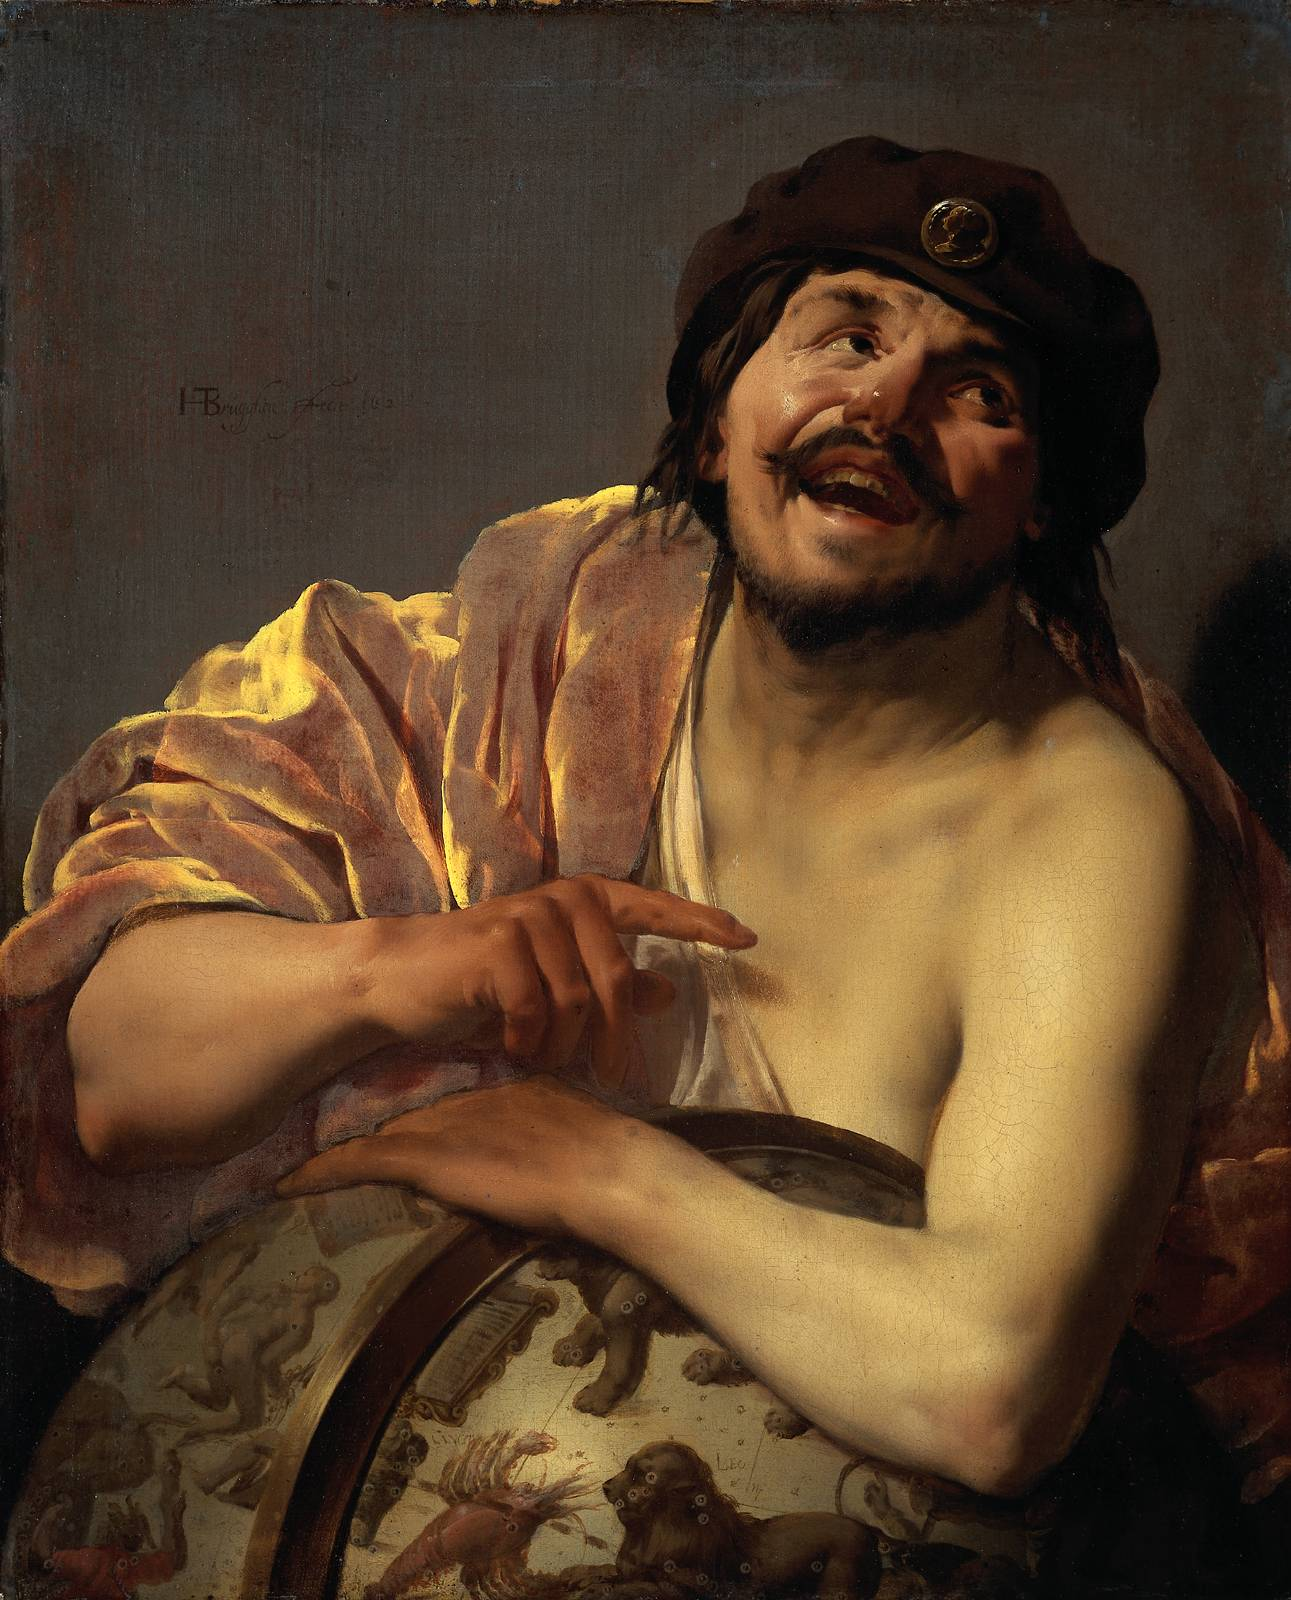
\includegraphics[width=0.4\linewidth]{../Chapter2/fig/democritus.jpg}
		\caption{Democritus}
		\label{fig:democritus}
	\end{subfigure}
	\caption{ Two greek philosophers, who made important philosophical
		contributions our understanding of matter. Empedocles (left), postulated the
		precursor to the elemental theory of matter ~\needcite{} and Democritus
		(right), postulated the precursor to the atomic theory of matter.  }
	\label{fig:atomists}
\end{figure}

Democritus was part of a movement of thought which was first to make the
intellectual jump that perhaps matter was not a continuum, but instead, composed
of 'atomon', small, indivisble particles which when configured togehter, created
all that is observable ~\needcite{}. Empedocles was making equally important
philosophical strides - in a manner complimentary to Democrits' opinion that
matter must be made of atomon, Empedocles argued that matter is composed of
elemental primatives ~\needcite{}.

Although Empedocles' 'periodic table' was only composed of Earth, Water, Fire,
and Air, the idea that some unseen transmutation of elemental forces might
generate observables in nature with quite different (but perhaps reminiscent)
properties then the 'pure substances' was an important step forward.
Proto-scientists were beginning to generate models which derived our complicated
observations, from simpler forms.

It took centuries of cultivation, leading up to the Scientific Revolution, for
the next great steps to occur, for science. Thankfully, the luminaries of the
Islamic Golden Age kept the fires of inqury burning ~\needcite{}.

\subsection{The Scientific Revolution}

Thanks to the mathematical foundations laid out, build, and maintained by the
minds of the Islamic Golden Age, Europe was well poised to reignite the flames
of scientific inquiry, during the post Renaissance Scientific Revolution
~\needcite{}.

This period of growth in science was unprecidented during the Scientific
Revolution, thanks to the seeds of empiricism germinated during the Islamic
Golden Age, fertilized by the Italian Renaissance, and helped to flourish
through British Empricism ~\needcite{}.

\begin{figure}[h]
	\centering
	\begin{subfigure}{.5\textwidth}
		\centering
		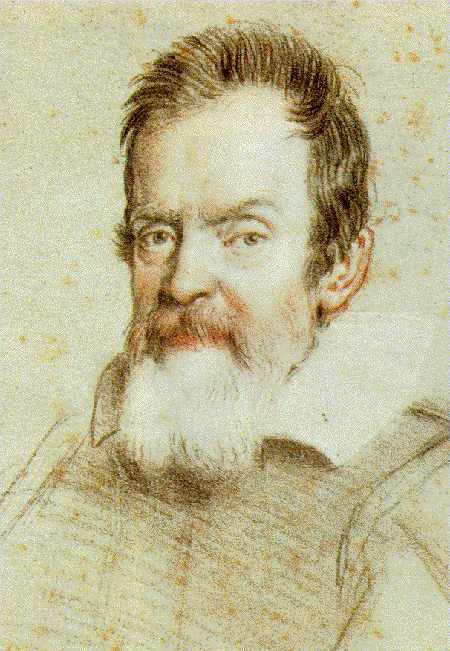
\includegraphics[width=0.4\linewidth]{../Chapter2/fig/galileo.jpg}
		\caption{Galileo}
		\label{fig:galileo}
	\end{subfigure}%
	\begin{subfigure}{0.5\textwidth}
		\centering
		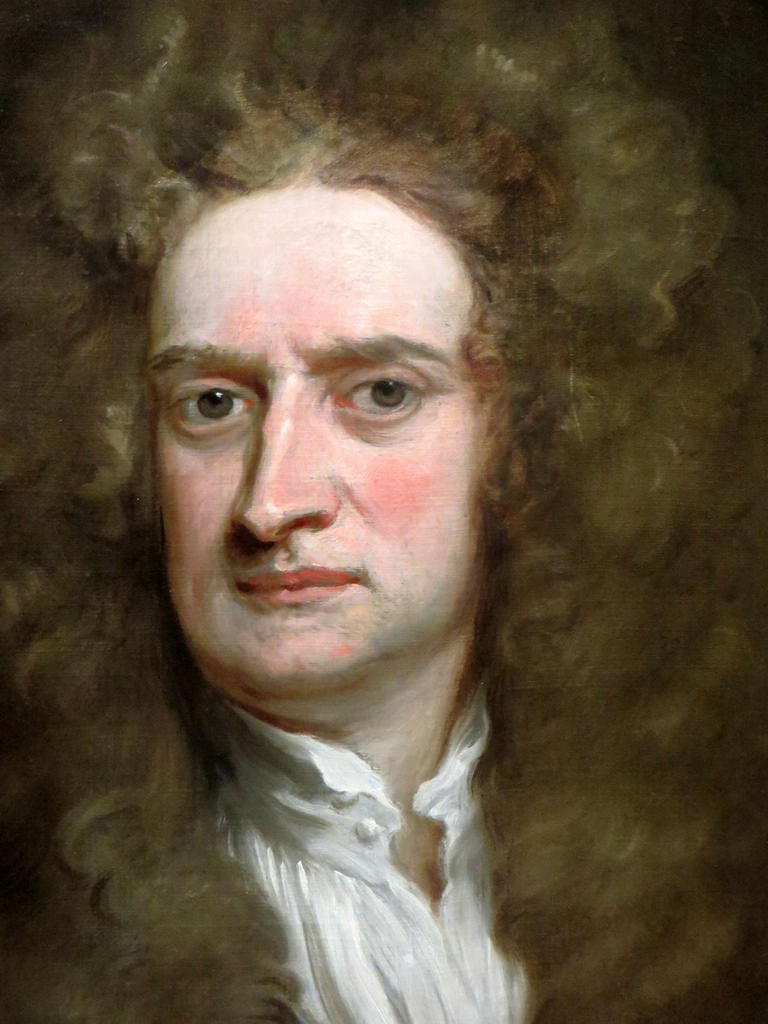
\includegraphics[width=0.4\linewidth]{../Chapter2/fig/newton.jpg}
		\caption{Newton}
		\label{fig:newton}
	\end{subfigure}
	\caption{ 
		Giants in the age of Empiricism, Newton~\ref{fig:newton} and
		Galileo~\ref{fig:galileo} both made foundational contributions to Physics.
		Galileo lived in Italy, born in 1564 and dying in 1642. Newton lived in
		England from 1642 until his death in 1727
	}
	\label{fig:atomists}
\end{figure}

\subsubsection{Galileo Galilei}
While Galileo is best known for his work in Observational Astronomy, his
importance to science extends beyond this. During his years in exile for his
controversial views of the heliocentric universe, he produced some of his most
important scientific work in kinematics ~\needcite{}. What made this work
remarkable is the care that Galileo took in merging careful mathematical
modeling with well designed experimentation. This methodical approach to inquiry
laid the foundation for others to slowly begin to pull back the curtains
obscuring physical law.

Galileo's formalization of the scientific method inexorably set science on a
course to delving deep into the nature of matter, and the laws of nature.

\subsubsection{Isaac Newton}
Fittingly born in the same year as Galileo's death, Isaac Newton would carry on
Galileo's legacy of rigorous mathematical modeling mixed with experimentaiton.
Perhaps no other scientist has touched so many different aspects of physics,
from theories of propegation of light, to celestial mechanics, to mathematics,
and kinematics.

Newton's Principia is perhaps the most important scientific work ever published.
It opened the doors of the universe in a way that nobody has since duplicated.
Newtons' laws of motion are still taught in school today, and although they have
since been shown to be inaccurate at the smallest and largest scales, they still
provide startlingly accurate predictions for the regular motion of matter.

One particularly tantelizing theory of Newton's was the corpuscular theory of
light. Although not his most influential theory by far, the idea that an
apparently continuous medium such as a beam of light might be made of small
packets of energy (corpuscules) turned out to be partially right ~\needcite{}.

Newton's theories, and contributions to science are enormous, and have moved us
deeper still into the underpinnings of matter. It would not be until roughly 200
years after his death, in the 19th century, that we finally can take the first
steps into the world of the atomic, and sub-atomic: the world of the proton. 

\subsection{Atomic Theory}

On the shoulders of giants such as Newton and Gallileo, science finally came to
know the tool which has been indispensable to modern particle physics:
scattering. Rutherford and Thompson both carried out the most important
scattering experiments in modern science, and provided us with the first hints
of a hidden, quantum world, though it would not be until the 20th century that
these important experiments would be fully contextualized with a theory of
quantum scattering.

Scattering experiments offer a very powerful method where we one uses a well
known initial state of matter (typically in the form of a beam), allows this
beam to interact with an unknown configuration of matter, and measures the
scattered beam. By carefully studying the kinematics of the scattered beam, we
can create models which allow us to understand the structure of the target
matter or describe the nature of the interaction between the beam and target. 

\subsubsection{Thompson}

\subsubsection{Rutherford}

\subsubsection{Dalton}

\subsection{Modern Quantum Physics: Quantum Electrodynamics and Quantum Chromodynamcs}

Gell-Mann, Sweig (8-fold way), Feynman, Wilczek, Weinberg, T Hooft, Parisano,
DGLAP. David Gross

Although Gell-Mann's simple quark model of baryons ~\needcite{} predicts the
correct quantiy for the spin of the proton, the work of Ashman et al (1988)
~\needcite{} at the European Muon Collaboraiton directly measured a portion of
the proton sturcture function $g_1$ and found that a rather small fraction of
the prton spin comes from quarks - and most of the spin is carried by the
gluons (Figure~\ref{fig:emc_g1_result}). 

\begin{figure}[H]
	\begin{center}
	
\includegraphics[width=0.5\linewidth]{../filler/squareimg.png}
	\caption{~\needfig{} ~\needcap{}. Results of EMC experiment showing that the structure
	function g1, tells us a thing about proton spin.}
	\label{fig:emc_g1_result}
\end{center}
\end{figure}

\subsubsection{Proton Spin Crisis}

\section{How to Model Proton Spin}
\begin{itemize}
		\item structure functions
		\item proton spin decomposition
		\item unpolarized parton distribution functions
		\item polarized parton distribution functions
		\item that sweet table from Delia hasch
		\item discussion $\bar{q}$, $q$, $L_q$, $g$
		\item DSSV figures
\end{itemize}
\section{How to Measure Proton Spin}
\begin{itemize}
		\item physics probes for proton spin
		\item W cross section
		\item derivation of Asymmetry
		\item kinematic extremes of Asymmetry
\end{itemize}
\subsection{Past Experimental Efforts}
\begin{itemize}
		\item summary of data on structure functions
		\item fixed target experiments
		\item collider experiments
\end{itemize}

\section{World Efforts to Measure Proton Spin}
\subsection{CERN}
\subsection{ZEUS}
\subsection{HERA}
\subsection{HERMES}
\subsection{COMPASS}
\subsection{EMC}
\subsection{SLAC}
\subsection{JLAB}

\section{Cross Sections and Luminosity}
\begin{itemize}
		\item vernier analysis note intro, equations
		\item summarize the papers on Lumoninosity
\end{itemize}

\chapter{Experimental Apparatus}

\chapter{Spin Analysis}



\chapter{The Vernier Analysis}



\chapter{Discussion and Conclusion}



\nocite{*}
% \singlespacing
% \bibliographystyle{alpha}
\bibliographystyle{plain}
\bibliography{bibliography}
\appendix

\section{First Thingie}

\section{Second Thingie}


\end{document}
